\chapter{Theoretical background}

\section{\textit{Rhodotorula toruloides}}

\textit{Rhodotorula toruloides} (previously \textit{Rhodosporidium toruloides}) is a non-conventional, oleaginous yeast, 
that can naturally accumulate
high amounts of lipids \cite{Rekena2023}. This yeast occurs naturally in leaves, soil, sea water, etc. It has a broad substrate range, 
which has made this yeast a popular for producing biological oils from inedible 
substrates such as pentose sugars and crude glycerol.\textit{R. toruloides} lipid fraction contains also carotenoid pigments, 
omega-3 linolenic acid and heptadecenoic acid,
which makes this yeast a promising organism for production of pharma- and nutraceuticals \cite{Tiukova2019}. 
It has been found that nitrogen limitation further induces lipid accumulation, 
65\% of lipids of dry cell weight were reached in a batch cultivation regime \cite{Rekena2023}.

One of the major determinants of the oleaginous phenotype of \textit{R. toruloides} is its capacity for acetylCoA production. 
Unlike non-oleaginous yeasts such as \textit{Saccharomyces cerevisiae}, \textit{R. toruloides} possesses the enzyme ATP-citrate lyase, 
which is the main source of acetyl-CoA for lipid
synthesis. Mitochondrial beta-oxidation pathway provides additional source of acetylCoA in this yeast. \cite{Tiukova2019}
Synthesis of acetyl-CoA from xylulose 5-phosphate by phosphoketolase (XPK), and the conversion of S-malate into pyruvate by 
malic enzyme (ME) that provides for NADPH enzymatic pathways also differ from the model yeast \textit{Saccharomyces
cerevisiae} and which specifically facilitate the generation of lipid precursors.\cite{Rekena2023}
Lipid biosynthetic reactions downstream of acetyl-CoA synthesis do not differ between oleaginous and non-oleaginous 
yeast species \cite{Tiukova2019}.

In \textit{R. toruloides} metabolic pathways producing acetyl-CoA and a cofactor NADPH
have been the main focus of metabolic studies due to their central role in lipid
biosynthesis. Fatty acids mainly accumulate as triacylglycerols (TAGs), and they are
produced via four enzymatic reactions that require 1 ATP and 2 NADPH molecules for adding 1 acetyl-CoA to the fatty acid chain.
Proteomics analysis has suggested that NADPH is primarily regenerated through the pentose phosphate pathway, when grown on xylose 
and glucose, but the role of malic enzyme is not clearly understood. The
role of XPK in the generation of acetyl-CoA has not been acknowledged previously, whereas
ACL has been demonstrated to be upregulated during lipid accumulation, especially in
presence of xylose.\cite{Rekena2023}


% \subsection{Physiological characteristics} % General Physiological characteristics

% \subsection{Central carbon metabolism}

\section{Overview of cellular growth laws}

\section{Genome-scale metabolic modeling} %incl. Constraint-based modeling, kinetic modeling, steady-state, limitations, e.g. regulation

A microorganism's phenotype can be described by its pattern of metabolic fluxes \cite{Kerkhoven2014}. Metabolic flux is the 
rate of turnover of molecules through a metabolic pathway. Flux is regulated by the enzymes involved in this pathway. Within cells, 
regulation of flux is vital for all metabolic pathways to regulate the pathway's activity under different conditions. \cite{Voet1995}

In biotechnology the aim is often to increase the capacity of specific fluxes. 
For this, metabolic engineering methods have been developed and many of these 
rely on balancing of intracellular metabolites using genome-scale models (GEMs) that in
combination with appropriate objective functions and constraints can be used to predict potential gene 
targets for obtaining a preferred flux distribution. \cite{Kerkhoven2014} 

Genome-scale metabolic models are comprehensive summaries of metabolic reactions of a
organism, which are derived from the organism's genome sequence \cite{Tiukova2019}. GEMs are organism specific and they account for genes,
 proteins, and biochemical reactions, which enable systematic
analysis of metabolism, where typically
the objective is to achieve a global picture of possible flux
patterns \cite{Kerkhoven2014}, \cite{Chen2023}. GEMs can be a powerful and helpful tool in metabolic studies, if their predictive 
power is
good \cite{Rekena2023}. They can be used for identification of potential metabolic engineering targets, or select the best
performing metabolic network among alternatives.
The first genome-scale model of \textit{R. toruloides} metabolism (rhto-GEM), includes 4869 genes, 
897 reactions, and 3334
metabolites. The simulation results confirmed that the \textit{R. toruloides} model provides valid growth predictions on glucose, 
xylose and glycerol. This makes rtho-GEM useful for future studies to improve the production of other
industrially important oleochemicals including both value-added fatty acids and carotenoids. \cite{Tiukova2019}

The reconstructed networks can be converted into mathematical stoichiometric matrices, where rows represent metabolites 
and columns represent individual reactions. This matrix will
determine the solution space of the metabolic network. GEMs are constrained by (1) the stoichiometry of the
network; (2) preset upper and lower boundaries for selected reactions (usually substrate uptake reactions,
but can also describe thermodynamics); and (3) the assumption of a steady state. \cite{Kerkhoven2014} Reconstruction of GEMs is shown in the figure 1.1.

\begin{figure}
    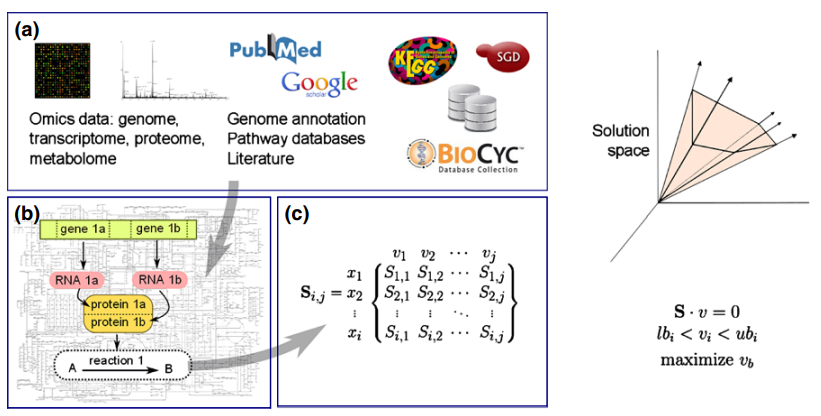
\includegraphics[width=\linewidth]{GEMs.png}
    \caption{Reconstruction of GEMs. (a) The genome annotation can be used 
    to reconstruct the metabolic network. (b) Gene-protein-reaction relationships are defined for the metabolic model. 
     (c). A solution space is defined from the constraints applied to the model and subsequent 
    analysis provides instructions for metabolic engineering strategies. This figure has been taken from article \cite{Kerkhoven2014}.}
    \label{GEMs}
\end{figure}

Steady state assumption
presumes that all the flux rates and metabolite concentrations are constant over time. In experiments this state can be
reached in chemostat cultivation and, in theory, during controlled batch logarithmic growth
phase when organisms grow at their maximum specific growth rate and the change of neither substrate concentration 
nor product formation will affect the growth regulation. \cite{Kerkhoven2014} 


\textbf{Constraint-based modeling}

Metabolism operates under countless of constraints. These include constraints that 
remain unchanged as they abide by the laws of physics (e.g. conservation of mass and energy, thermodynamics), 
and constraints that can vary by organism, environmental condition, the state of the 
cell (e.g. nutrient uptake rate, biomass composition), and constraints that can also change through evolution or 
changes in gene expression [Citation]. %\cite{Kerkhoven2022}

A major limitation in the predictive power of conventional GEMs is that they ignore the capacity of a 
cell to support a metabolic flux is constrained by its resource allocation, as most metabolic reactions are 
catalyzed by enzymes. The synthesis of enzymes is resource- and energy-expensive, their catalytic 
capacities are limited by their kinetics, also the quantity of enzymes is space-constraint, such that 
stringency in resource allocation is vital for optimal cell growth. The modeling problem of resource allocation can 
be narrowly defined by only considering protein allocation: “given a certain budget, what is the best way to distribute 
it”, where budget refers to the total cellular protein level that is distributed over all its constituent proteins. [Citation] %\cite{Kerkhoven2022}

This means that an increase in the requirement of an enzyme or a pathway would be a trade-off for other
functions. Experimental evidence indicates that for various organisms resource re-allocation could be an effective strategy 
in response to nutrient and growth shift, which demonstrates the biological significance 
of proteome constraints. \cite{Chen2023} 
Applying such constraints in a metabolism model reduces simulated flux distributions to those that are most 
economic and also limits the phenotypes that the model can simulate. These both contribute to more realistic results. 
Such models have already found numerous applications in e.g. unraveling the underlying mechanisms for observed metabolic 
phenotypes and the prediction of strain optimization strategies.[Citation] %\cite{Kerkhoven2022}
This suggests that proteome constraints could be a valuable addition to GEMs to
improve model predictions \cite{Chen2023}. 

The first approach that allows for a direct incorporation of proteomics data to account for enzyme limitation
was the GECKO framework. The GECKO method is built on the principle that any metabolic reaction flux has a
biologically natural constraint equal to the intracellular enzyme concentration multiplied by
the enzyme's turnover number ($k_{cat}$). In metabolic network, the enzyme constraint is
defined as maximum rate of enzymatic reaction ($v_{max}$) that the metabolic flux cannot exceed. [Citation] %\Alina MSc thesis

Enzyme-constrained GEMs integrate additional constraints on enzyme capacity and
their total abundances. Phenomenological constraint is imposed on metabolic flux (v; mmol/gDCW/h), formulated as enzyme
kinetics: $v <=  E \cdot k_{cat}$, where $E$ is protein abundance (mmol/gDCW) and $k_{cat}$ is the enzyme's turnover number (1/s),
provided with an upper limit on individual or total protein abundances. The integration of
enzymatic constraints in \textit{S. cerevisiae} has significantly improved phenotype prediction. \cite{Rekena2023}


\textbf{Flux balance analysis}

% GEMs can simulate metabolic flux distributions by optimization of an objective function that describes the 
% perceived cellular objective that propels 
% metabolism, by flux balance analysis (FBA). %\cite{Kerkhoven2022}

Flux balance analysis (FBA) is commonly used for adding additional constraints, where an
assumed biological objective is applied in the form of maximizing (or minimizing) a certain flux. This results in
a solution in the solution space that satisfies the presumed objective. The most commonly used objective function is maximization of the 
specific growth rate, ATP generation or product formation. FBA is often used for estimating the biotechnological potential of 
microorganisms and pinpoint genetic manipulations that could improve the performance of a cell. The main applications of 
FBA are:
(1) Instructions for metabolic engineering purposes;
(2) Biological interpretation and discovery through
contextualizing high-throughput data;
(3) Development of a computational framework;
(4) Evolutionary elucidation;
(5) Description of multispecies communities. \cite{Kerkhoven2014}

% The simplest approach to consider the economics of 
% resource allocation assumes that cells aim to minimize 
% the number of active fluxes to yield the most efficient 
% flux distribution. Parsimonious FBA is an example of a computational approach that can find such minimal 
% flux distributions by removing loops and thereby partially alleviates the protein allocation problem, but more 
% advanced approaches have since been developed. %\cite{Kerkhoven2022}

% GEMs and FBA can be applied to identify potential metabolic engineering strategies, or even select the best 
% performing network among alternatives. There have been
% several successful examples where genome-scale constraint-based modeling was applied for strain improvement. \cite{Kerkhoven2014}

% While GEMs can predict the best performing engineering strategies based on the metabolic network, the application 
% of those changes may not be as straightforward,
% as metabolic networks are highly regulated at various levels to ensure the robustness of the functional system. 
% Predictions of allosteric regulation, functional state of
% enzymes (post-transcriptional modifications) are currently
% not taken into account in GEMs. Additionally, enzyme
% kinetics and performance of non-native genes/proteins are
% currently not covered in GEMs. Although the first genome-scale and reduced constraint-based models that take
% regulation into account have emerged for \textit{E. coli}, they have so far only been
% created for certain regulatory systems present in yeast. Although the lack of regulatory
% predicting power in GEMs hinders the quality of predictions for metabolic engineering purposes, the combination of 
% modeling data with real experiments can precisely
% identify the regions which are highly regulated at post-transcriptional level and allows one to investigate those
% regions more thoroughly using bottom-up approaches. \cite{Kerkhoven2014}


% \textbf{Kinetic modeling}

% GEMs follow a top-down approach of systems biology,
% where information from the different layers of the system
% (genome, transcriptome, metabolome, etc.) are integrated
% to construct a comprehensive view of metabolism, and
% insight is gained by studying the behavior of this system
% as a whole (Bruggeman and Westerhoff, 2007). Contrastingly, a bottom-up approach assumes that the behavior of a
% system can be deduced from the characteristics of its constitutive parts (Bruggeman and Westerhoff, 2007). The
% interactions of these parts give rise to the behavior of the
% system, and therefore, a good understanding of the parts
% of the system is paramount. Models of metabolism that
% follow this paradigm are called kinetic models, and the
% constitutive parts of this system are the enzymes, their
% metabolites, other effectors, and their interactions. The
% separation of models of metabolism between top-down
% and bottom-up is not completely black and white, as it is
% now also possible to construct kinetic models on a genomic scale, as detailed below. \cite{Kerkhoven2014}

% Kinetic modeling of metabolism has essentially evolved
% out of the fields of molecular biology and enzymology,
% moving from characterizing one enzyme in isolation to
% investigating them in the biological context of a metabolic pathway. The combination of the S-matrix and the v-vector that
% describe the kinetic model results in a set of ordinary differential equations (ODEs) that describe the dynamics of
% the metabolite (dX) over time (dt) (Fig. 2). These models
% can subsequently be used in a variety of ways to address
% different questions regarding metabolism, such as how to
% increase or reduce the yield of a particular (by-)product
% (Table 1). In light of metabolic engineering, of particular
% interest is the analysis of flux control, while these models
% can also be used for the evaluation of different engineering strategies.\cite{Kerkhoven2014}

% \textbf{Steady-state}

% \textbf{Limitations}

% GEMs and kinetic models both have their advantages
% and drawbacks. GEMs are comprehensive but are dependent on a pseudosteady state and in their current form
% do not take regulation, such as gene-protein and protein-protein level interactions, allosteric regulation or 
% regulation at post-translational level, into account. At the same
% time, kinetic models require parameter values that are
% difficult to estimate at the global scale. As neither of them
% can fully replace the other, there has been a considerable
% effort on combining these two approaches in a singular
% model or applying them in succession. GEMs in combination with global datasets are invaluable for detecting
% the metabolic bottlenecks, but due to lack of kinetic data
% about enzyme activities or regulation mechanisms they
% are limited in their predictive power. Applying kinetic models on metabolic bottlenecks previously detected with
% GEMs can help to understand the regulation or kinetics
% of these specific enzymatic steps, as one would not need
% model parameters for the whole system (Fig. 3). \cite{Kerkhoven2014}

% GEMs allow the calculation of
% metabolic fluxes that represent activity of different metabolic pathways under specified conditions,
% e.g., an uptake of a particular carbon source. Flux balance analysis predicted
% that up to 87\% of NADPH was regenerated from xylose through the oxidative part of pentose
% phosphate pathway (oxPPP). Phosphoketolase was suggested as the main supplier of acetyl-CoA 
% during lipogenesis in xylose-grown cells. On the other hand, TCA cycle related
% enzymes were suggested for NADPH production on acetate-grown cells, demonstrating
% that metabolic operations can vary significantly with the carbon source uptake. Models have
% also been used to study metabolism during cell growth on glucose and glycerol. A better understanding 
% of how different metabolic pathways contribute to lipid accumulation under different substrates would help to 
% design better metabolic engineering strategies. \cite{Rekena2023}

% \textbf{Regulation}





\section{Overview of microbial cultivation methods}




